% Options for packages loaded elsewhere
% Options for packages loaded elsewhere
\PassOptionsToPackage{unicode}{hyperref}
\PassOptionsToPackage{hyphens}{url}
\PassOptionsToPackage{dvipsnames,svgnames,x11names}{xcolor}
%
\documentclass[
  french,
  letterpaper,
  DIV=11,
  numbers=noendperiod]{scrartcl}
\usepackage{xcolor}
\usepackage{amsmath,amssymb}
\setcounter{secnumdepth}{5}
\usepackage{iftex}
\ifPDFTeX
  \usepackage[T1]{fontenc}
  \usepackage[utf8]{inputenc}
  \usepackage{textcomp} % provide euro and other symbols
\else % if luatex or xetex
  \usepackage{unicode-math} % this also loads fontspec
  \defaultfontfeatures{Scale=MatchLowercase}
  \defaultfontfeatures[\rmfamily]{Ligatures=TeX,Scale=1}
\fi
\usepackage{lmodern}
\ifPDFTeX\else
  % xetex/luatex font selection
\fi
% Use upquote if available, for straight quotes in verbatim environments
\IfFileExists{upquote.sty}{\usepackage{upquote}}{}
\IfFileExists{microtype.sty}{% use microtype if available
  \usepackage[]{microtype}
  \UseMicrotypeSet[protrusion]{basicmath} % disable protrusion for tt fonts
}{}
\makeatletter
\@ifundefined{KOMAClassName}{% if non-KOMA class
  \IfFileExists{parskip.sty}{%
    \usepackage{parskip}
  }{% else
    \setlength{\parindent}{0pt}
    \setlength{\parskip}{6pt plus 2pt minus 1pt}}
}{% if KOMA class
  \KOMAoptions{parskip=half}}
\makeatother
% Make \paragraph and \subparagraph free-standing
\makeatletter
\ifx\paragraph\undefined\else
  \let\oldparagraph\paragraph
  \renewcommand{\paragraph}{
    \@ifstar
      \xxxParagraphStar
      \xxxParagraphNoStar
  }
  \newcommand{\xxxParagraphStar}[1]{\oldparagraph*{#1}\mbox{}}
  \newcommand{\xxxParagraphNoStar}[1]{\oldparagraph{#1}\mbox{}}
\fi
\ifx\subparagraph\undefined\else
  \let\oldsubparagraph\subparagraph
  \renewcommand{\subparagraph}{
    \@ifstar
      \xxxSubParagraphStar
      \xxxSubParagraphNoStar
  }
  \newcommand{\xxxSubParagraphStar}[1]{\oldsubparagraph*{#1}\mbox{}}
  \newcommand{\xxxSubParagraphNoStar}[1]{\oldsubparagraph{#1}\mbox{}}
\fi
\makeatother

\usepackage{color}
\usepackage{fancyvrb}
\newcommand{\VerbBar}{|}
\newcommand{\VERB}{\Verb[commandchars=\\\{\}]}
\DefineVerbatimEnvironment{Highlighting}{Verbatim}{commandchars=\\\{\}}
% Add ',fontsize=\small' for more characters per line
\usepackage{framed}
\definecolor{shadecolor}{RGB}{241,243,245}
\newenvironment{Shaded}{\begin{snugshade}}{\end{snugshade}}
\newcommand{\AlertTok}[1]{\textcolor[rgb]{0.68,0.00,0.00}{#1}}
\newcommand{\AnnotationTok}[1]{\textcolor[rgb]{0.37,0.37,0.37}{#1}}
\newcommand{\AttributeTok}[1]{\textcolor[rgb]{0.40,0.45,0.13}{#1}}
\newcommand{\BaseNTok}[1]{\textcolor[rgb]{0.68,0.00,0.00}{#1}}
\newcommand{\BuiltInTok}[1]{\textcolor[rgb]{0.00,0.23,0.31}{#1}}
\newcommand{\CharTok}[1]{\textcolor[rgb]{0.13,0.47,0.30}{#1}}
\newcommand{\CommentTok}[1]{\textcolor[rgb]{0.37,0.37,0.37}{#1}}
\newcommand{\CommentVarTok}[1]{\textcolor[rgb]{0.37,0.37,0.37}{\textit{#1}}}
\newcommand{\ConstantTok}[1]{\textcolor[rgb]{0.56,0.35,0.01}{#1}}
\newcommand{\ControlFlowTok}[1]{\textcolor[rgb]{0.00,0.23,0.31}{\textbf{#1}}}
\newcommand{\DataTypeTok}[1]{\textcolor[rgb]{0.68,0.00,0.00}{#1}}
\newcommand{\DecValTok}[1]{\textcolor[rgb]{0.68,0.00,0.00}{#1}}
\newcommand{\DocumentationTok}[1]{\textcolor[rgb]{0.37,0.37,0.37}{\textit{#1}}}
\newcommand{\ErrorTok}[1]{\textcolor[rgb]{0.68,0.00,0.00}{#1}}
\newcommand{\ExtensionTok}[1]{\textcolor[rgb]{0.00,0.23,0.31}{#1}}
\newcommand{\FloatTok}[1]{\textcolor[rgb]{0.68,0.00,0.00}{#1}}
\newcommand{\FunctionTok}[1]{\textcolor[rgb]{0.28,0.35,0.67}{#1}}
\newcommand{\ImportTok}[1]{\textcolor[rgb]{0.00,0.46,0.62}{#1}}
\newcommand{\InformationTok}[1]{\textcolor[rgb]{0.37,0.37,0.37}{#1}}
\newcommand{\KeywordTok}[1]{\textcolor[rgb]{0.00,0.23,0.31}{\textbf{#1}}}
\newcommand{\NormalTok}[1]{\textcolor[rgb]{0.00,0.23,0.31}{#1}}
\newcommand{\OperatorTok}[1]{\textcolor[rgb]{0.37,0.37,0.37}{#1}}
\newcommand{\OtherTok}[1]{\textcolor[rgb]{0.00,0.23,0.31}{#1}}
\newcommand{\PreprocessorTok}[1]{\textcolor[rgb]{0.68,0.00,0.00}{#1}}
\newcommand{\RegionMarkerTok}[1]{\textcolor[rgb]{0.00,0.23,0.31}{#1}}
\newcommand{\SpecialCharTok}[1]{\textcolor[rgb]{0.37,0.37,0.37}{#1}}
\newcommand{\SpecialStringTok}[1]{\textcolor[rgb]{0.13,0.47,0.30}{#1}}
\newcommand{\StringTok}[1]{\textcolor[rgb]{0.13,0.47,0.30}{#1}}
\newcommand{\VariableTok}[1]{\textcolor[rgb]{0.07,0.07,0.07}{#1}}
\newcommand{\VerbatimStringTok}[1]{\textcolor[rgb]{0.13,0.47,0.30}{#1}}
\newcommand{\WarningTok}[1]{\textcolor[rgb]{0.37,0.37,0.37}{\textit{#1}}}

\usepackage{longtable,booktabs,array}
\newcounter{none} % for unnumbered tables
\usepackage{calc} % for calculating minipage widths
% Correct order of tables after \paragraph or \subparagraph
\usepackage{etoolbox}
\makeatletter
\patchcmd\longtable{\par}{\if@noskipsec\mbox{}\fi\par}{}{}
\makeatother
% Allow footnotes in longtable head/foot
\IfFileExists{footnotehyper.sty}{\usepackage{footnotehyper}}{\usepackage{footnote}}
\makesavenoteenv{longtable}
\usepackage{graphicx}
\makeatletter
\newsavebox\pandoc@box
\newcommand*\pandocbounded[1]{% scales image to fit in text height/width
  \sbox\pandoc@box{#1}%
  \Gscale@div\@tempa{\textheight}{\dimexpr\ht\pandoc@box+\dp\pandoc@box\relax}%
  \Gscale@div\@tempb{\linewidth}{\wd\pandoc@box}%
  \ifdim\@tempb\p@<\@tempa\p@\let\@tempa\@tempb\fi% select the smaller of both
  \ifdim\@tempa\p@<\p@\scalebox{\@tempa}{\usebox\pandoc@box}%
  \else\usebox{\pandoc@box}%
  \fi%
}
% Set default figure placement to htbp
\def\fps@figure{htbp}
\makeatother


% definitions for citeproc citations
\NewDocumentCommand\citeproctext{}{}
\NewDocumentCommand\citeproc{mm}{%
  \begingroup\def\citeproctext{#2}\cite{#1}\endgroup}
\makeatletter
 % allow citations to break across lines
 \let\@cite@ofmt\@firstofone
 % avoid brackets around text for \cite:
 \def\@biblabel#1{}
 \def\@cite#1#2{{#1\if@tempswa , #2\fi}}
\makeatother
\newlength{\cslhangindent}
\setlength{\cslhangindent}{1.5em}
\newlength{\csllabelwidth}
\setlength{\csllabelwidth}{3em}
\newenvironment{CSLReferences}[2] % #1 hanging-indent, #2 entry-spacing
 {\begin{list}{}{%
  \setlength{\itemindent}{0pt}
  \setlength{\leftmargin}{0pt}
  \setlength{\parsep}{0pt}
  % turn on hanging indent if param 1 is 1
  \ifodd #1
   \setlength{\leftmargin}{\cslhangindent}
   \setlength{\itemindent}{-1\cslhangindent}
  \fi
  % set entry spacing
  \setlength{\itemsep}{#2\baselineskip}}}
 {\end{list}}
\usepackage{calc}
\newcommand{\CSLBlock}[1]{\hfill\break\parbox[t]{\linewidth}{\strut\ignorespaces#1\strut}}
\newcommand{\CSLLeftMargin}[1]{\parbox[t]{\csllabelwidth}{\strut#1\strut}}
\newcommand{\CSLRightInline}[1]{\parbox[t]{\linewidth - \csllabelwidth}{\strut#1\strut}}
\newcommand{\CSLIndent}[1]{\hspace{\cslhangindent}#1}

\ifLuaTeX
\usepackage[bidi=basic,shorthands=off]{babel}
\else
\usepackage[bidi=default,shorthands=off]{babel}
\fi
\ifLuaTeX
  \usepackage{selnolig} % disable illegal ligatures
\fi


\setlength{\emergencystretch}{3em} % prevent overfull lines

\providecommand{\tightlist}{%
  \setlength{\itemsep}{0pt}\setlength{\parskip}{0pt}}



 


\KOMAoption{captions}{tableheading}
\makeatletter
\@ifpackageloaded{caption}{}{\usepackage{caption}}
\AtBeginDocument{%
\ifdefined\contentsname
  \renewcommand*\contentsname{Table des matières}
\else
  \newcommand\contentsname{Table des matières}
\fi
\ifdefined\listfigurename
  \renewcommand*\listfigurename{Liste des Figures}
\else
  \newcommand\listfigurename{Liste des Figures}
\fi
\ifdefined\listtablename
  \renewcommand*\listtablename{Liste des Tables}
\else
  \newcommand\listtablename{Liste des Tables}
\fi
\ifdefined\figurename
  \renewcommand*\figurename{Figure}
\else
  \newcommand\figurename{Figure}
\fi
\ifdefined\tablename
  \renewcommand*\tablename{Table}
\else
  \newcommand\tablename{Table}
\fi
}
\@ifpackageloaded{float}{}{\usepackage{float}}
\floatstyle{ruled}
\@ifundefined{c@chapter}{\newfloat{codelisting}{h}{lop}}{\newfloat{codelisting}{h}{lop}[chapter]}
\floatname{codelisting}{Listing}
\newcommand*\listoflistings{\listof{codelisting}{Liste des Listings}}
\makeatother
\makeatletter
\makeatother
\makeatletter
\@ifpackageloaded{caption}{}{\usepackage{caption}}
\@ifpackageloaded{subcaption}{}{\usepackage{subcaption}}
\makeatother
\usepackage{bookmark}
\IfFileExists{xurl.sty}{\usepackage{xurl}}{} % add URL line breaks if available
\urlstyle{same}
\hypersetup{
  pdftitle={Clustering},
  pdfauthor={Oscar JOSEPH--GENESLAY},
  pdflang={fr},
  colorlinks=true,
  linkcolor={blue},
  filecolor={Maroon},
  citecolor={Blue},
  urlcolor={Blue},
  pdfcreator={LaTeX via pandoc}}


\title{Clustering}
\author{Oscar JOSEPH--GENESLAY}
\date{}
\begin{document}
\maketitle

\renewcommand*\contentsname{Table des matières}
{
\setcounter{tocdepth}{3}
\tableofcontents
}

\section{L'article}\label{larticle}

Ce fichier \textbf{Quarto} utilise cet article Flynt et Dean (2016),
l'objectif est de reproduire les résultats obtenus sur le sujet du
clustering. Dans cette étude, on explore les méthodes de clustering en
se basant sur des données simulées, en ayant pour objectif de
reconstituer le clustering avec des méthodes statistiques.

\section{Génération des données
simulées}\label{guxe9nuxe9ration-des-donnuxe9es-simuluxe9es}

\subsubsection{Importation des packages}\label{importation-des-packages}

\begin{Shaded}
\begin{Highlighting}[]
\FunctionTok{library}\NormalTok{(mvtnorm)}
\FunctionTok{library}\NormalTok{(MASS)}
\FunctionTok{library}\NormalTok{(dplyr)}
\FunctionTok{library}\NormalTok{(ggplot2)}
\FunctionTok{library}\NormalTok{(plot3D)}
\FunctionTok{library}\NormalTok{(gplots)}
\FunctionTok{library}\NormalTok{(tidyverse)}
\FunctionTok{library}\NormalTok{(plotly)}
\FunctionTok{library}\NormalTok{(tidyverse)}
\FunctionTok{library}\NormalTok{(scales)}
\FunctionTok{library}\NormalTok{(factoextra)}
\FunctionTok{library}\NormalTok{(NbClust)}
\end{Highlighting}
\end{Shaded}

\subparagraph{Répartition des points
simulés}\label{ruxe9partition-des-points-simuluxe9s}

\begin{Shaded}
\begin{Highlighting}[]
\FunctionTok{set.seed}\NormalTok{(}\DecValTok{288}\NormalTok{)}

\CommentTok{\# Creating continuous variables}
\NormalTok{pi }\OtherTok{=} \FunctionTok{c}\NormalTok{(}\FloatTok{0.3}\NormalTok{, }\FloatTok{0.4}\NormalTok{, }\FloatTok{0.3}\NormalTok{)}
\NormalTok{mu }\OtherTok{=} \FunctionTok{matrix}\NormalTok{(}\FunctionTok{c}\NormalTok{(}\DecValTok{0}\NormalTok{, }\DecValTok{0}\NormalTok{, }\DecValTok{3}\NormalTok{, }\DecValTok{5}\NormalTok{, }\DecValTok{0}\NormalTok{, }\DecValTok{6}\NormalTok{), }\DecValTok{2}\NormalTok{, }\DecValTok{3}\NormalTok{, }\AttributeTok{byrow=}\ConstantTok{FALSE}\NormalTok{) }\CommentTok{\# Définition des moyennes des groupes 2 par 2}
\NormalTok{Sigma.sph }\OtherTok{=} \FunctionTok{diag}\NormalTok{(}\FunctionTok{c}\NormalTok{(}\DecValTok{1}\NormalTok{, }\DecValTok{1}\NormalTok{))}
\NormalTok{Sigma.ell }\OtherTok{=} \FunctionTok{matrix}\NormalTok{(}\FunctionTok{c}\NormalTok{(}\DecValTok{2}\NormalTok{, }\FloatTok{1.3}\NormalTok{, }\FloatTok{1.3}\NormalTok{, }\DecValTok{1}\NormalTok{),}\DecValTok{2}\NormalTok{, }\DecValTok{2}\NormalTok{, }\AttributeTok{byrow=}\ConstantTok{TRUE}\NormalTok{)}
\NormalTok{cl }\OtherTok{=} \FunctionTok{sample}\NormalTok{(}\FunctionTok{c}\NormalTok{(}\DecValTok{1}\NormalTok{, }\DecValTok{2}\NormalTok{, }\DecValTok{3}\NormalTok{), }\DecValTok{600}\NormalTok{, T, pi)}
\NormalTok{X }\OtherTok{=} \FunctionTok{matrix}\NormalTok{(}\DecValTok{0}\NormalTok{, }\DecValTok{600}\NormalTok{, }\DecValTok{2}\NormalTok{)}
\ControlFlowTok{for}\NormalTok{(i }\ControlFlowTok{in} \DecValTok{1}\SpecialCharTok{:}\DecValTok{600}\NormalTok{)}
\NormalTok{\{}
  \FunctionTok{ifelse}\NormalTok{(cl[i] }\SpecialCharTok{==} \DecValTok{3}\NormalTok{, X[i,]}\OtherTok{\textless{}{-}}\FunctionTok{rmvnorm}\NormalTok{(}\DecValTok{1}\NormalTok{, mu[,}\DecValTok{3}\NormalTok{], Sigma.ell), X[i,]}\OtherTok{\textless{}{-}}\FunctionTok{rmvnorm}\NormalTok{(}\DecValTok{1}\NormalTok{, mu[,cl[i]], Sigma.sph))}
\NormalTok{\}}
\FunctionTok{eqscplot}\NormalTok{(X, }\AttributeTok{col =} \StringTok{"gray1"}\NormalTok{, }\AttributeTok{pch =} \DecValTok{18}\NormalTok{)}
\end{Highlighting}
\end{Shaded}

\pandocbounded{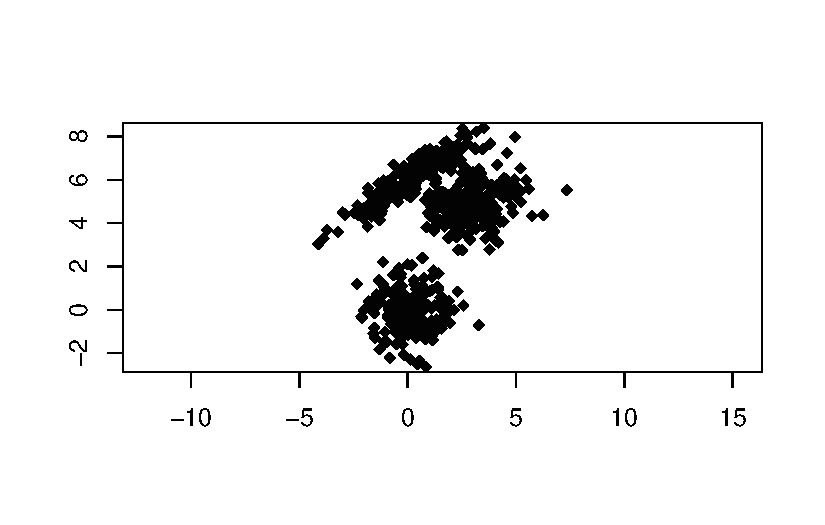
\includegraphics[keepaspectratio]{cluster_analysis_files/figure-pdf/unnamed-chunk-2-1.pdf}}

\subparagraph{Répartition des points simulés - version
ggplot}\label{ruxe9partition-des-points-simuluxe9s---version-ggplot}

\begin{Shaded}
\begin{Highlighting}[]
\NormalTok{X }\SpecialCharTok{\%\textgreater{}\%} \FunctionTok{as\_tibble}\NormalTok{() }\SpecialCharTok{\%\textgreater{}\%} \FunctionTok{ggplot}\NormalTok{(}\FunctionTok{aes}\NormalTok{(}\AttributeTok{x =}\NormalTok{ V1, }\AttributeTok{y=}\NormalTok{ V2)) }\SpecialCharTok{+} 
  \FunctionTok{geom\_point}\NormalTok{() }\SpecialCharTok{+} \FunctionTok{theme\_minimal}\NormalTok{() }\SpecialCharTok{+} \FunctionTok{ggtitle}\NormalTok{(}\StringTok{"Répartition des points simulés en 2 dimensions"}\NormalTok{)}
\end{Highlighting}
\end{Shaded}

\pandocbounded{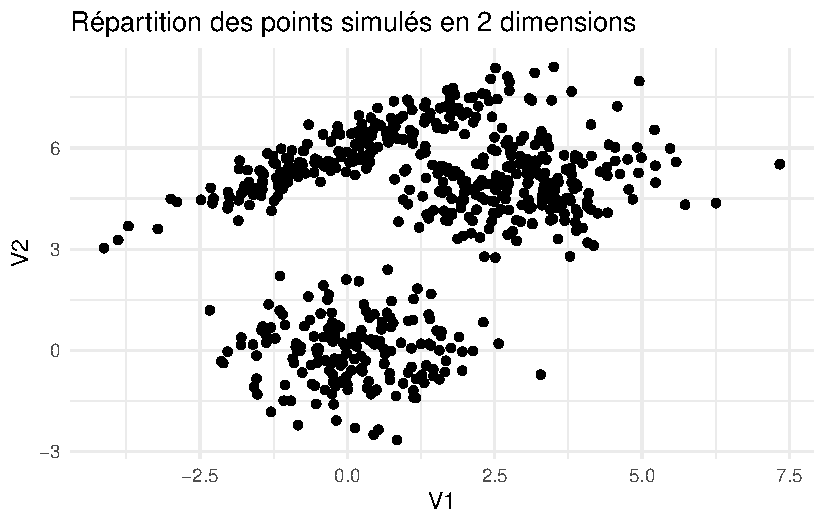
\includegraphics[keepaspectratio]{cluster_analysis_files/figure-pdf/unnamed-chunk-3-1.pdf}}

\subparagraph{Représentation en 3D de l'histogramme de la loi normale
bivariée}\label{repruxe9sentation-en-3d-de-lhistogramme-de-la-loi-normale-bivariuxe9e}

\begin{Shaded}
\begin{Highlighting}[]
\CommentTok{\# 1. Créer les "bins" (les classes) pour les deux colonnes}
\NormalTok{x\_bins }\OtherTok{\textless{}{-}} \FunctionTok{cut}\NormalTok{(X[,}\DecValTok{1}\NormalTok{], }\AttributeTok{breaks =} \DecValTok{10}\NormalTok{)}
\NormalTok{y\_bins }\OtherTok{\textless{}{-}} \FunctionTok{cut}\NormalTok{(X[,}\DecValTok{2}\NormalTok{], }\AttributeTok{breaks =} \DecValTok{10}\NormalTok{)}

\CommentTok{\# 2. Créer la table de fréquences (la matrice Z)}
\NormalTok{z\_matrix }\OtherTok{\textless{}{-}} \FunctionTok{table}\NormalTok{(x\_bins, y\_bins)}

\CommentTok{\# 3. Définir les coordonnées des centres des barres}
\NormalTok{x\_coords }\OtherTok{\textless{}{-}} \FunctionTok{seq}\NormalTok{(}\FunctionTok{min}\NormalTok{(X[,}\DecValTok{1}\NormalTok{]), }\FunctionTok{max}\NormalTok{(X[,}\DecValTok{1}\NormalTok{]), }\AttributeTok{length.out =} \FunctionTok{nrow}\NormalTok{(z\_matrix))}
\NormalTok{y\_coords }\OtherTok{\textless{}{-}} \FunctionTok{seq}\NormalTok{(}\FunctionTok{min}\NormalTok{(X[,}\DecValTok{2}\NormalTok{]), }\FunctionTok{max}\NormalTok{(X[,}\DecValTok{2}\NormalTok{]), }\AttributeTok{length.out =} \FunctionTok{ncol}\NormalTok{(z\_matrix))}

\FunctionTok{hist3D}\NormalTok{(}\AttributeTok{x =}\NormalTok{ x\_coords, }\AttributeTok{y =}\NormalTok{ y\_coords, }\AttributeTok{z =}\NormalTok{ z\_matrix,}
       \AttributeTok{border =} \StringTok{"black"}\NormalTok{, }
       \AttributeTok{colkey =} \ConstantTok{TRUE}\NormalTok{, }
       \AttributeTok{lighting =} \ConstantTok{TRUE}\NormalTok{, }
       \AttributeTok{main =} \StringTok{"Représentation 3D de la loi normale bivariée"}\NormalTok{,}
       \AttributeTok{xlab =} \StringTok{"x"}\NormalTok{, }
       \AttributeTok{ylab =} \StringTok{"y"}\NormalTok{, }
       \AttributeTok{zlab =} \StringTok{"Fréquence"}\NormalTok{,}
       \AttributeTok{phi =} \DecValTok{50}\NormalTok{, }\AttributeTok{theta =} \SpecialCharTok{{-}}\DecValTok{30}\NormalTok{) }\CommentTok{\# Angles de vue}
\end{Highlighting}
\end{Shaded}

\pandocbounded{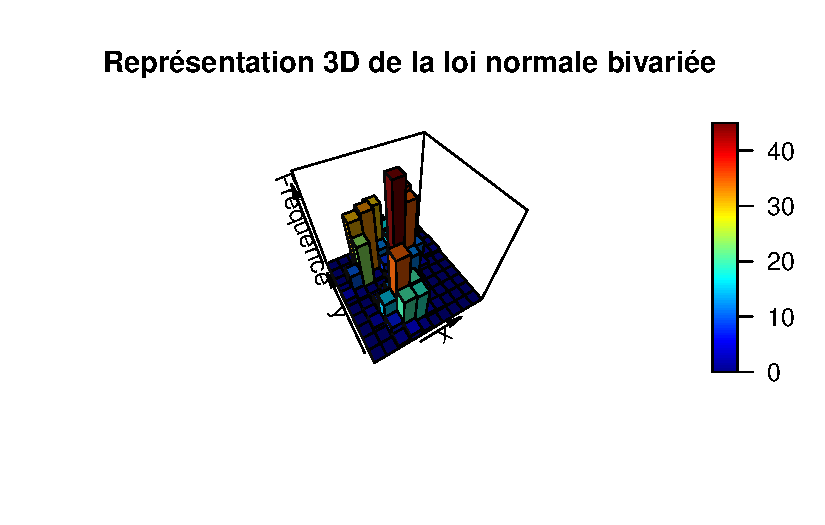
\includegraphics[keepaspectratio]{cluster_analysis_files/figure-pdf/unnamed-chunk-4-1.pdf}}

\subparagraph{Répartition des
individus}\label{ruxe9partition-des-individus}

\textbf{Groupe 1}

On a 177 noirs (29,5\%), 237 rouges (39,5\%), 186 vert (31\%).

On est dans une loi normale bivariée, de paramètre (Espérance, Matrice
variance-covariance). De moyenne = (0,0) et de matrice variance
covariance = marice identité :

\begin{Shaded}
\begin{Highlighting}[]
\FunctionTok{diag}\NormalTok{(}\DecValTok{2}\NormalTok{)}
\end{Highlighting}
\end{Shaded}

\begin{verbatim}
     [,1] [,2]
[1,]    1    0
[2,]    0    1
\end{verbatim}

\textbf{Groupe 2}

On a une moyenne (3,5)

\textbf{Groupe 3}

On a une moyenne (0,6), et une matrice (2, 1.3, 1.3, 1)

\begin{Shaded}
\begin{Highlighting}[]
\FunctionTok{prop.table}\NormalTok{(}\FunctionTok{table}\NormalTok{(cl))}
\end{Highlighting}
\end{Shaded}

\begin{verbatim}
cl
    1     2     3 
0.295 0.395 0.310 
\end{verbatim}

\subsubsection{Représentation des données simulées en fonction de leur
groupe}\label{repruxe9sentation-des-donnuxe9es-simuluxe9es-en-fonction-de-leur-groupe}

\begin{Shaded}
\begin{Highlighting}[]
\FunctionTok{as\_tibble}\NormalTok{(X) }\SpecialCharTok{\%\textgreater{}\%} \FunctionTok{ggplot}\NormalTok{(}\FunctionTok{aes}\NormalTok{(}\AttributeTok{x =}\NormalTok{ V1, }\AttributeTok{y=}\NormalTok{V2)) }\SpecialCharTok{+} \FunctionTok{geom\_point}\NormalTok{(}\AttributeTok{color =}\NormalTok{ cl) }\SpecialCharTok{+} \FunctionTok{theme\_minimal}\NormalTok{() }\SpecialCharTok{+} \FunctionTok{ggtitle}\NormalTok{(}\StringTok{"Représentation des variables continues en fonction des groupes prédéfinis"}\NormalTok{) }\OtherTok{{-}\textgreater{}}\NormalTok{ graph1}
\NormalTok{graph1}
\end{Highlighting}
\end{Shaded}

\pandocbounded{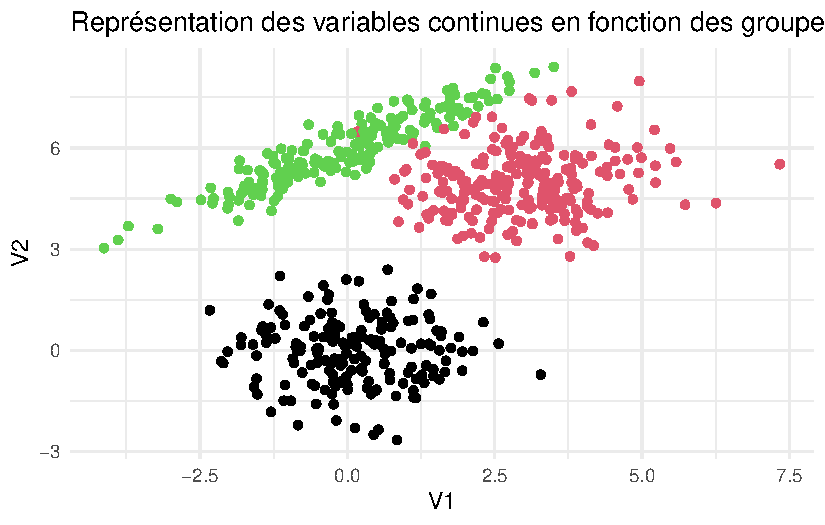
\includegraphics[keepaspectratio]{cluster_analysis_files/figure-pdf/unnamed-chunk-7-1.pdf}}

\subsection{Création des variables
discrètes}\label{cruxe9ation-des-variables-discruxe8tes}

c1 : il utilise rbinom pour générer 600 chiffres avec une proba de
succès de 0.5, +1 pour mettre les valeurs à 1 ou 2

c2 : si la couleur du point est noir alors on applique une proba plus
importante au succès 1 sinon on applique une proba plus importante au
succès 2.

\begin{Shaded}
\begin{Highlighting}[]
\CommentTok{\# Creating discrete variables}
\CommentTok{\# Note for poLCA and clustMD, coding must start at 1.}

\CommentTok{\# Uniform prob. of success for all observations (success means a value of 2, whereas failure would be a value of 1)}
\NormalTok{c1 }\OtherTok{=} \FunctionTok{rbinom}\NormalTok{(}\DecValTok{600}\NormalTok{, }\DecValTok{1}\NormalTok{, .}\DecValTok{5}\NormalTok{) }\SpecialCharTok{+} \DecValTok{1}

\CommentTok{\# Success more likely in red and green groups}
\NormalTok{c2 }\OtherTok{=} \ConstantTok{NULL}
\ControlFlowTok{for}\NormalTok{(i }\ControlFlowTok{in} \DecValTok{1}\SpecialCharTok{:}\DecValTok{600}\NormalTok{)\{}
  \FunctionTok{ifelse}\NormalTok{(cl[i] }\SpecialCharTok{==} \DecValTok{1}\NormalTok{, c2[i]}\OtherTok{\textless{}{-}}\FunctionTok{rbinom}\NormalTok{(}\DecValTok{1}\NormalTok{, }\DecValTok{1}\NormalTok{, .}\DecValTok{1}\NormalTok{)}\SpecialCharTok{+}\DecValTok{1}\NormalTok{, c2[i]}\OtherTok{\textless{}{-}}\FunctionTok{rbinom}\NormalTok{(}\DecValTok{1}\NormalTok{, }\DecValTok{1}\NormalTok{, .}\DecValTok{9}\NormalTok{)}\SpecialCharTok{+}\DecValTok{1}\NormalTok{)}
\NormalTok{\}}

\CommentTok{\# More likely to be a 1 in black, a 2 in red and a 3 in green}
\NormalTok{c3 }\OtherTok{=} \ConstantTok{NULL}
\ControlFlowTok{for}\NormalTok{(i }\ControlFlowTok{in} \DecValTok{1}\SpecialCharTok{:}\DecValTok{600}\NormalTok{)\{}
  \ControlFlowTok{if}\NormalTok{(cl[i] }\SpecialCharTok{==} \DecValTok{1}\NormalTok{) c3[i] }\OtherTok{=} \FunctionTok{sample}\NormalTok{(}\DecValTok{1}\SpecialCharTok{:}\DecValTok{3}\NormalTok{, }\DecValTok{1}\NormalTok{, }\AttributeTok{prob =} \FunctionTok{c}\NormalTok{(.}\DecValTok{6}\NormalTok{, .}\DecValTok{2}\NormalTok{, .}\DecValTok{2}\NormalTok{))}
  \ControlFlowTok{if}\NormalTok{(cl[i] }\SpecialCharTok{==} \DecValTok{2}\NormalTok{) c3[i] }\OtherTok{=} \FunctionTok{sample}\NormalTok{(}\DecValTok{1}\SpecialCharTok{:}\DecValTok{3}\NormalTok{, }\DecValTok{1}\NormalTok{, }\AttributeTok{prob =} \FunctionTok{c}\NormalTok{(.}\DecValTok{1}\NormalTok{, .}\DecValTok{8}\NormalTok{, .}\DecValTok{1}\NormalTok{))}
  \ControlFlowTok{if}\NormalTok{(cl[i] }\SpecialCharTok{==} \DecValTok{3}\NormalTok{) c3[i] }\OtherTok{=} \FunctionTok{sample}\NormalTok{(}\DecValTok{1}\SpecialCharTok{:}\DecValTok{3}\NormalTok{, }\DecValTok{1}\NormalTok{, }\AttributeTok{prob =} \FunctionTok{c}\NormalTok{(.}\DecValTok{1}\NormalTok{, .}\DecValTok{1}\NormalTok{, .}\DecValTok{8}\NormalTok{))}
\NormalTok{\}}


\CommentTok{\# Success more likely in red group}
\NormalTok{c4 }\OtherTok{=} \ConstantTok{NULL}
\ControlFlowTok{for}\NormalTok{(i }\ControlFlowTok{in} \DecValTok{1}\SpecialCharTok{:}\DecValTok{600}\NormalTok{)\{}
  \FunctionTok{ifelse}\NormalTok{(cl[i] }\SpecialCharTok{==} \DecValTok{2}\NormalTok{, c4[i]}\OtherTok{\textless{}{-}}\FunctionTok{rbinom}\NormalTok{(}\DecValTok{1}\NormalTok{, }\DecValTok{1}\NormalTok{, .}\DecValTok{8}\NormalTok{)}\SpecialCharTok{+}\DecValTok{1}\NormalTok{, c4[i]}\OtherTok{\textless{}{-}}\FunctionTok{rbinom}\NormalTok{(}\DecValTok{1}\NormalTok{, }\DecValTok{1}\NormalTok{, .}\DecValTok{2}\NormalTok{)}\SpecialCharTok{+}\DecValTok{1}\NormalTok{)}
\NormalTok{\}}

\CommentTok{\# Merging the variables into our complete mixed{-}mode dataset, vars}
\NormalTok{vars }\OtherTok{=} \FunctionTok{cbind}\NormalTok{(X, c1, c2, c3, c4)}
\FunctionTok{head}\NormalTok{(vars)}
\end{Highlighting}
\end{Shaded}

\begin{verbatim}
                           c1 c2 c3 c4
[1,]  1.6137555  4.6784541  1  2  2  2
[2,]  0.3135524 -0.3026124  2  1  2  1
[3,]  3.1383011  3.7670414  2  2  2  1
[4,] -1.5400580 -0.1531943  1  1  1  1
[5,]  2.5165331  4.8541686  1  2  2  1
[6,]  1.9779610  4.4491698  1  2  2  2
\end{verbatim}

\subparagraph{Fréquence des modalités dans chaque groupe et variable des
données}\label{fruxe9quence-des-modalituxe9s-dans-chaque-groupe-et-variable-des-donnuxe9es}

\begin{Shaded}
\begin{Highlighting}[]
\NormalTok{df\_plot }\OtherTok{\textless{}{-}}\NormalTok{ vars[, }\DecValTok{3}\SpecialCharTok{:}\DecValTok{6}\NormalTok{] }\SpecialCharTok{\%\textgreater{}\%} 
  \FunctionTok{as\_tibble}\NormalTok{() }\SpecialCharTok{\%\textgreater{}\%} 
  \FunctionTok{mutate}\NormalTok{(}\AttributeTok{cl =} \FunctionTok{as.factor}\NormalTok{(cl)) }\SpecialCharTok{\%\textgreater{}\%} 
  \FunctionTok{pivot\_longer}\NormalTok{(}\AttributeTok{cols =} \FunctionTok{c}\NormalTok{(c1, c2, c3, c4), }\AttributeTok{names\_to =} \StringTok{"groupe"}\NormalTok{, }\AttributeTok{values\_to =} \StringTok{"valeur"}\NormalTok{) }\SpecialCharTok{\%\textgreater{}\%} 
  \FunctionTok{mutate}\NormalTok{(}\AttributeTok{valeur =} \FunctionTok{as.factor}\NormalTok{(valeur))}

\CommentTok{\# Création du graphique style "publication"}
\FunctionTok{ggplot}\NormalTok{(df\_plot, }\FunctionTok{aes}\NormalTok{(}\AttributeTok{x =}\NormalTok{ cl, }\AttributeTok{fill =}\NormalTok{ valeur)) }\SpecialCharTok{+} 
  \CommentTok{\# Barres 100\% empilées, avec un léger contour pour bien les séparer si besoin}
  \FunctionTok{geom\_bar}\NormalTok{(}\AttributeTok{position =} \StringTok{"fill"}\NormalTok{, }\AttributeTok{width =} \FloatTok{0.8}\NormalTok{) }\SpecialCharTok{+} 
  
  \CommentTok{\# Séparation par groupe (c1, c2, c3, c4)}
  \FunctionTok{facet\_grid}\NormalTok{(}\SpecialCharTok{\textasciitilde{}}\NormalTok{ groupe) }\SpecialCharTok{+} \FunctionTok{scale\_fill\_manual}\NormalTok{(}\AttributeTok{values =} \FunctionTok{c}\NormalTok{(}\StringTok{"grey30"}\NormalTok{, }\StringTok{"grey65"}\NormalTok{, }\StringTok{"grey90"}\NormalTok{))}\SpecialCharTok{+}
  \FunctionTok{theme\_classic}\NormalTok{()}\SpecialCharTok{+}
  \FunctionTok{ggtitle}\NormalTok{(}\StringTok{"Fréquence des modalités dans chaque groupe et variable des données"}\NormalTok{)}
\end{Highlighting}
\end{Shaded}

\pandocbounded{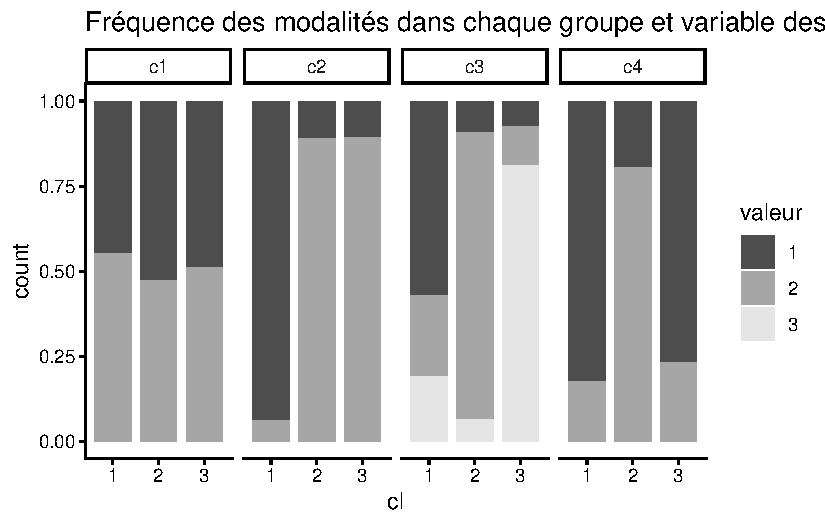
\includegraphics[keepaspectratio]{cluster_analysis_files/figure-pdf/unnamed-chunk-9-1.pdf}}

\subsubsection{Application de la fonction
k-means}\label{application-de-la-fonction-k-means}

On aurait pu explorer toutes les possiblités pour 2 clusters mais c'est
impossible vu le nombre de possibilités

\begin{Shaded}
\begin{Highlighting}[]
\FunctionTok{library}\NormalTok{(kStatistics)}
\FunctionTok{nStirling2}\NormalTok{(}\DecValTok{600}\NormalTok{, }\DecValTok{2}\NormalTok{)}
\end{Highlighting}
\end{Shaded}

\begin{verbatim}
[1] 2.074758e+180
\end{verbatim}

\subsection{Méthode du coude}\label{muxe9thode-du-coude}

\begin{Shaded}
\begin{Highlighting}[]
\CommentTok{\# Elbow method}
\FunctionTok{fviz\_nbclust}\NormalTok{(vars [,}\DecValTok{1}\SpecialCharTok{:}\DecValTok{2}\NormalTok{], kmeans, }\AttributeTok{method =} \StringTok{"wss"}\NormalTok{) }\SpecialCharTok{+}
    \FunctionTok{geom\_vline}\NormalTok{(}\AttributeTok{xintercept =} \DecValTok{3}\NormalTok{, }\AttributeTok{linetype =} \DecValTok{2}\NormalTok{)}\SpecialCharTok{+}
  \FunctionTok{labs}\NormalTok{(}\AttributeTok{subtitle =} \StringTok{"Méthode du coude {-} Nombre optimal de clusters"}\NormalTok{) }
\end{Highlighting}
\end{Shaded}

\begin{verbatim}
Warning: The `size` argument of `element_line()` is deprecated as of ggplot2 3.4.0.
i Please use the `linewidth` argument instead.
i The deprecated feature was likely used in the ggpubr package.
  Please report the issue at <https://github.com/kassambara/ggpubr/issues>.
\end{verbatim}

\begin{verbatim}
Warning: The `size` argument of `element_rect()` is deprecated as of ggplot2 3.4.0.
i Please use the `linewidth` argument instead.
i The deprecated feature was likely used in the ggpubr package.
  Please report the issue at <https://github.com/kassambara/ggpubr/issues>.
\end{verbatim}

\begin{verbatim}
Warning: Using `size` aesthetic for lines was deprecated in ggplot2 3.4.0.
i Please use `linewidth` instead.
i The deprecated feature was likely used in the ggpubr package.
  Please report the issue at <https://github.com/kassambara/ggpubr/issues>.
\end{verbatim}

\pandocbounded{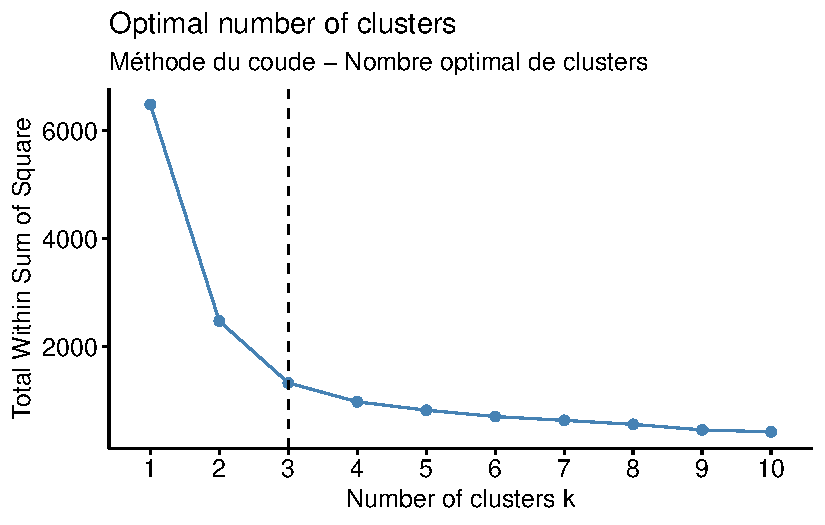
\includegraphics[keepaspectratio]{cluster_analysis_files/figure-pdf/unnamed-chunk-11-1.pdf}}

\begin{Shaded}
\begin{Highlighting}[]
\FunctionTok{fviz\_nbclust}\NormalTok{(vars [,}\DecValTok{1}\SpecialCharTok{:}\DecValTok{2}\NormalTok{], kmeans, }\AttributeTok{nstart =} \DecValTok{25}\NormalTok{, }\AttributeTok{method =} \StringTok{"gap\_stat"}\NormalTok{, }\AttributeTok{nboot =} \DecValTok{50}\NormalTok{)}\SpecialCharTok{+}
\FunctionTok{labs}\NormalTok{(}\AttributeTok{subtitle =} \StringTok{"Gap statistic method"}\NormalTok{) }
\end{Highlighting}
\end{Shaded}

\begin{verbatim}
Warning: pas de convergence en 10 itérations
\end{verbatim}

\begin{verbatim}
Warning: `aes_string()` was deprecated in ggplot2 3.0.0.
i Please use tidy evaluation idioms with `aes()`.
i See also `vignette("ggplot2-in-packages")` for more information.
i The deprecated feature was likely used in the factoextra package.
  Please report the issue at <https://github.com/kassambara/factoextra/issues>.
\end{verbatim}

\pandocbounded{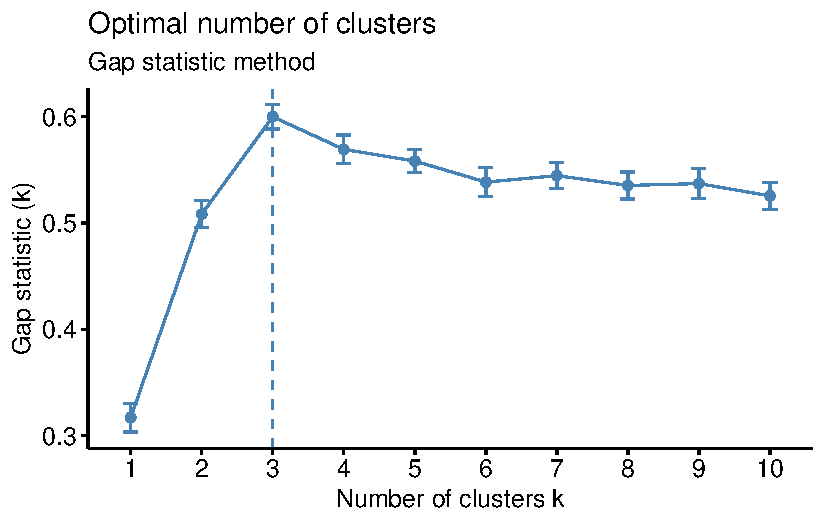
\includegraphics[keepaspectratio]{cluster_analysis_files/figure-pdf/unnamed-chunk-12-1.pdf}}

\subsubsection{kmeans - Hartigan}\label{kmeans---hartigan}

\textbf{Algo d'Hartigan}

Description de l'algorithme d'Hartigam pour la méthode des kmeans.

\[
\begin{array}{l}
\textbf{Algorithme de Hartigan-Wong (K-Means)} \\
\hline
1.\ \textbf{Initialisation : } \text{Distribuer chaque point dans un cluster au hasard.} \\
2.\ \textbf{Calcul des centres : } \text{Calculer le centre moyen de chaque groupe formé.} \\
3.\ \textbf{Boucle principale : } \text{Pour chaque point du jeu de données :} \\
\quad 4.\ \textbf{Test de transfert : } \text{Calculer si déplacer le point vers un autre groupe} \\
\quad \quad \text{rend l'ensemble des clusters plus compact.} \\
\quad 5.\ \textbf{Décision : } \text{Si le transfert améliore la qualité globale :} \\
\quad \quad 6.\ \textbf{Action : } \text{Déplacer le point dans le nouveau groupe immédiatement.} \\
\quad \quad 7.\ \textbf{Mise à jour : } \text{Recalculer aussitôt le centre du groupe qui a perdu} \\
\quad \quad \quad \text{le point et celui du groupe qui l'a gagné.} \\
8.\ \textbf{Convergence : } \text{Recommencer l'étape 3 tant que des points bougent encore.} \\
\hline
\end{array}
\]

\begin{Shaded}
\begin{Highlighting}[]
\FunctionTok{library}\NormalTok{(gridExtra)}
\NormalTok{cluster1 }\OtherTok{=} \FunctionTok{kmeans}\NormalTok{ (vars [,}\DecValTok{1}\SpecialCharTok{:}\DecValTok{2}\NormalTok{], }\DecValTok{1}\NormalTok{, }\AttributeTok{nstart =} \DecValTok{50}\NormalTok{) }
\NormalTok{cluster2 }\OtherTok{=} \FunctionTok{kmeans}\NormalTok{ (vars [,}\DecValTok{1}\SpecialCharTok{:}\DecValTok{2}\NormalTok{], }\DecValTok{2}\NormalTok{, }\AttributeTok{nstart =} \DecValTok{50}\NormalTok{) }\CommentTok{\# dans k1 il y a 181 individus / dans k2 il y en a 419}
\NormalTok{cluster3 }\OtherTok{=} \FunctionTok{kmeans}\NormalTok{ (vars [,}\DecValTok{1}\SpecialCharTok{:}\DecValTok{2}\NormalTok{], }\DecValTok{3}\NormalTok{, }\AttributeTok{nstart =} \DecValTok{50}\NormalTok{)}

\FunctionTok{library}\NormalTok{(tidyverse)}
\CommentTok{\# Point moyen : moyenne\_1 \& moyenne\_2}
\FunctionTok{as\_tibble}\NormalTok{(vars[,}\DecValTok{1}\SpecialCharTok{:}\DecValTok{2}\NormalTok{]) }\SpecialCharTok{\%\textgreater{}\%} \FunctionTok{summarise}\NormalTok{(}\AttributeTok{moyenne\_1 =} \FunctionTok{mean}\NormalTok{(V1),}
                         \AttributeTok{moyenne\_2 =} \FunctionTok{mean}\NormalTok{(V2),}
                         \AttributeTok{Variance =}\NormalTok{ (}\FunctionTok{var}\NormalTok{(V1) }\SpecialCharTok{+} \FunctionTok{var}\NormalTok{(V2)) }\SpecialCharTok{*} \DecValTok{599} \CommentTok{\# Somme des distances euclidiennes par rapport au p.m,}
\NormalTok{                         ) }
\end{Highlighting}
\end{Shaded}

\begin{verbatim}
# A tibble: 1 x 3
  moyenne_1 moyenne_2 Variance
      <dbl>     <dbl>    <dbl>
1      1.18      3.79    6481.
\end{verbatim}

\begin{Shaded}
\begin{Highlighting}[]
\FunctionTok{as\_tibble}\NormalTok{(X) }\SpecialCharTok{\%\textgreater{}\%} \FunctionTok{ggplot}\NormalTok{(}\FunctionTok{aes}\NormalTok{(}\AttributeTok{x =}\NormalTok{ V1, }\AttributeTok{y=}\NormalTok{V2)) }\SpecialCharTok{+} \FunctionTok{geom\_point}\NormalTok{(}\AttributeTok{color =}\NormalTok{ cluster3}\SpecialCharTok{$}\NormalTok{cluster) }\SpecialCharTok{+} \FunctionTok{theme\_minimal}\NormalTok{() }\SpecialCharTok{+} \FunctionTok{ggtitle}\NormalTok{(}\StringTok{"Représentation des variables continues en fonction des groupes prédéfinis"}\NormalTok{) }\OtherTok{{-}\textgreater{}}\NormalTok{ graph2}

\FunctionTok{grid.arrange}\NormalTok{(graph1, graph2, }\AttributeTok{nrow =} \DecValTok{1}\NormalTok{)}
\end{Highlighting}
\end{Shaded}

\pandocbounded{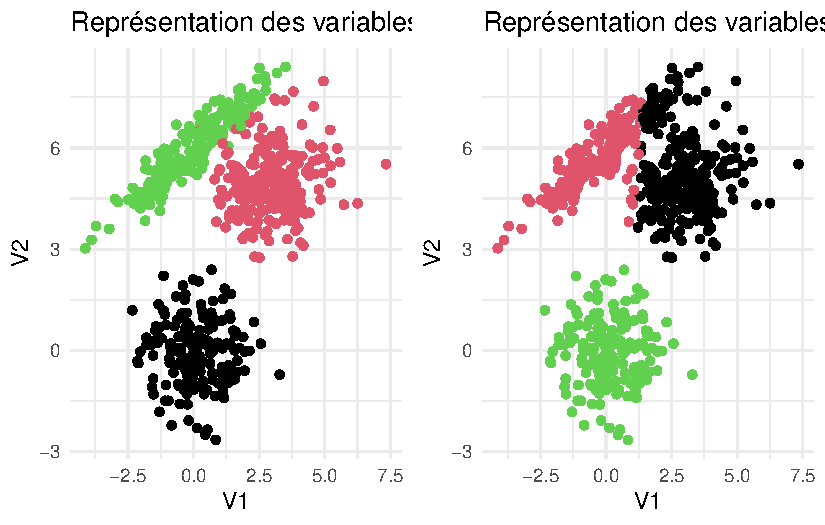
\includegraphics[keepaspectratio]{cluster_analysis_files/figure-pdf/unnamed-chunk-13-1.pdf}}

\subsubsection{kmeans - Lloyd}\label{kmeans---lloyd}

\textbf{Algo de Lloyd}

\[
\begin{array}{l}
\textbf{Algorithme de Lloyd (K-Means)} \\
\hline
1.\ \textbf{Initialisation : } \text{Choisir } k \text{ points au hasard pour être les centres.} \\
2.\ \textbf{Boucle principale : } \textbf{Répéter tant qu'il y a des changements :} \\
\quad 3.\ \textbf{Assignation globale : } \text{Chaque point choisit le centre le plus} \\
\quad \quad \text{proche sans se soucier des autres points.} \\
\quad 4.\ \textbf{Attente : } \text{On attend que TOUS les points aient choisi leur groupe.} \\
\quad 5.\ \textbf{Mise à jour groupée : } \text{Une fois que tout le monde a fini de bouger,} \\
\quad \quad \text{on recalcule tous les nouveaux centres en une seule fois.} \\
6.\ \textbf{Convergence : } \text{Arrêter quand les centres ne bougent plus d'une étape à l'autre.} \\
\hline
\end{array}
\]

\begin{Shaded}
\begin{Highlighting}[]
\NormalTok{cluster3\_lloyd }\OtherTok{=} \FunctionTok{kmeans}\NormalTok{ (vars [,}\DecValTok{1}\SpecialCharTok{:}\DecValTok{2}\NormalTok{], }\DecValTok{3}\NormalTok{, }\AttributeTok{nstart =} \DecValTok{50}\NormalTok{, }\AttributeTok{algorithm =} \StringTok{"Lloyd"}\NormalTok{)}
\end{Highlighting}
\end{Shaded}

\begin{verbatim}
Warning: pas de convergence en 10 itérations
Warning: pas de convergence en 10 itérations
Warning: pas de convergence en 10 itérations
Warning: pas de convergence en 10 itérations
Warning: pas de convergence en 10 itérations
Warning: pas de convergence en 10 itérations
Warning: pas de convergence en 10 itérations
Warning: pas de convergence en 10 itérations
Warning: pas de convergence en 10 itérations
Warning: pas de convergence en 10 itérations
Warning: pas de convergence en 10 itérations
Warning: pas de convergence en 10 itérations
Warning: pas de convergence en 10 itérations
\end{verbatim}

\begin{Shaded}
\begin{Highlighting}[]
\FunctionTok{as\_tibble}\NormalTok{(X) }\SpecialCharTok{\%\textgreater{}\%} \FunctionTok{ggplot}\NormalTok{(}\FunctionTok{aes}\NormalTok{(}\AttributeTok{x =}\NormalTok{ V1, }\AttributeTok{y=}\NormalTok{V2)) }\SpecialCharTok{+} \FunctionTok{geom\_point}\NormalTok{(}\AttributeTok{color =}\NormalTok{ cluster3\_lloyd}\SpecialCharTok{$}\NormalTok{cluster) }\SpecialCharTok{+} \FunctionTok{theme\_minimal}\NormalTok{() }\SpecialCharTok{+} \FunctionTok{ggtitle}\NormalTok{(}\StringTok{"Représentation des variables continues en fonction des groupes prédéfinis"}\NormalTok{)}
\end{Highlighting}
\end{Shaded}

\pandocbounded{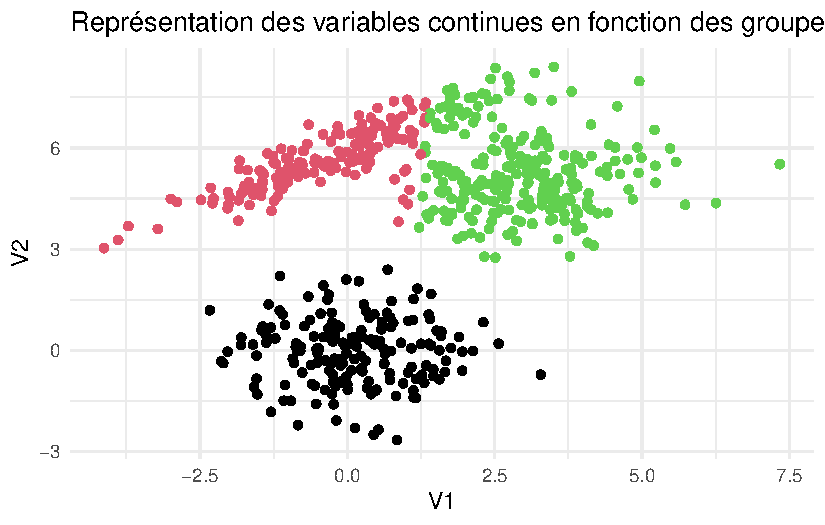
\includegraphics[keepaspectratio]{cluster_analysis_files/figure-pdf/unnamed-chunk-14-1.pdf}}

\subsubsection{Représentation de l'enveloppe
convexe}\label{repruxe9sentation-de-lenveloppe-convexe}

\begin{Shaded}
\begin{Highlighting}[]
\CommentTok{\# 1. Combiner vos données, la couleur d\textquotesingle{}origine (cl) et les résultats du k{-}means}
\NormalTok{df }\OtherTok{\textless{}{-}} \FunctionTok{as\_tibble}\NormalTok{(X) }\SpecialCharTok{\%\textgreater{}\%}
  \FunctionTok{mutate}\NormalTok{(}
    \AttributeTok{Couleur\_Origine =}\NormalTok{ cl,}
    \CommentTok{\# On extrait les affectations aux clusters de l\textquotesingle{}objet kmeans en facteur}
    \AttributeTok{Cluster\_Kmeans =} \FunctionTok{as.factor}\NormalTok{(cluster3\_lloyd}\SpecialCharTok{$}\NormalTok{cluster) }
\NormalTok{  )}

\CommentTok{\# 2. Calculer les points formant l\textquotesingle{}enveloppe convexe pour CHAQUE cluster k{-}means}
\CommentTok{\# La fonction chull() renvoie les indices des points qui forment la bordure convexe}
\NormalTok{hulls }\OtherTok{\textless{}{-}}\NormalTok{ df }\SpecialCharTok{\%\textgreater{}\%}
  \FunctionTok{group\_by}\NormalTok{(Cluster\_Kmeans) }\SpecialCharTok{\%\textgreater{}\%}
  \FunctionTok{slice}\NormalTok{(}\FunctionTok{chull}\NormalTok{(V1, V2))}

\CommentTok{\# 3. Créer le graphique combiné}
\FunctionTok{ggplot}\NormalTok{(df, }\FunctionTok{aes}\NormalTok{(}\AttributeTok{x =}\NormalTok{ V1, }\AttributeTok{y =}\NormalTok{ V2)) }\SpecialCharTok{+}
  \CommentTok{\# Étape A : Tracer les enveloppes convexes (polygones) des K{-}means}
  \CommentTok{\# alpha = 0.3 permet de rendre la surface transparente pour voir les points}
  \FunctionTok{geom\_polygon}\NormalTok{(}\AttributeTok{data =}\NormalTok{ hulls, }
               \FunctionTok{aes}\NormalTok{(}\AttributeTok{fill =}\NormalTok{ Cluster\_Kmeans, }\AttributeTok{group =}\NormalTok{ Cluster\_Kmeans), }
               \AttributeTok{alpha =} \FloatTok{0.3}\NormalTok{, }\AttributeTok{color =} \StringTok{"black"}\NormalTok{, }\AttributeTok{linetype =} \StringTok{"dashed"}\NormalTok{) }\SpecialCharTok{+}
  \FunctionTok{scale\_fill\_manual}\NormalTok{(}\AttributeTok{values =} \FunctionTok{c}\NormalTok{(}\StringTok{"\#FAADAD"}\NormalTok{, }\StringTok{"\#ADB4FA"}\NormalTok{, }\StringTok{"\#ADFABA"}\NormalTok{))}\SpecialCharTok{+}
               
  \CommentTok{\# Étape B : Tracer les points avec leurs couleurs d\textquotesingle{}origine (groupes prédéfinis)}
  \FunctionTok{geom\_point}\NormalTok{(}\FunctionTok{aes}\NormalTok{(}\AttributeTok{color =} \FunctionTok{factor}\NormalTok{(Couleur\_Origine))) }\SpecialCharTok{+}
  
  \CommentTok{\# Esthétique}
  \FunctionTok{theme\_minimal}\NormalTok{() }\SpecialCharTok{+}
  \FunctionTok{ggtitle}\NormalTok{(}\StringTok{"Représentation des variables continues en fonction des groupes prédéfinis}\SpecialCharTok{\textbackslash{}n}\StringTok{et enveloppes convexes des K{-}means"}\NormalTok{) }\SpecialCharTok{+}
  \FunctionTok{labs}\NormalTok{(}\AttributeTok{fill =} \StringTok{"Clusters K{-}means"}\NormalTok{, }\AttributeTok{color =} \StringTok{"Groupes initiaux"}\NormalTok{) }
\end{Highlighting}
\end{Shaded}

\pandocbounded{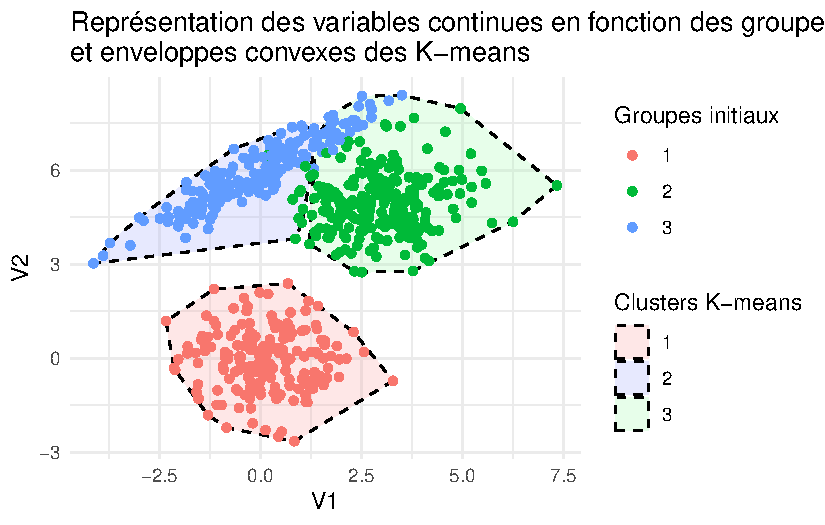
\includegraphics[keepaspectratio]{cluster_analysis_files/figure-pdf/unnamed-chunk-15-1.pdf}}

\begin{Shaded}
\begin{Highlighting}[]
\FunctionTok{fviz\_cluster}\NormalTok{(cluster3\_lloyd, }
             \AttributeTok{data =}\NormalTok{ vars[, }\DecValTok{1}\SpecialCharTok{:}\DecValTok{2}\NormalTok{], }
             \AttributeTok{ellipse.type =} \StringTok{"convex"}\NormalTok{,}
             \AttributeTok{geom =} \StringTok{"point"}\NormalTok{, }\CommentTok{\# "point" évite d\textquotesingle{}afficher le numéro de chaque ligne}
             \AttributeTok{show.clust.cent =} \ConstantTok{TRUE}\NormalTok{, }\CommentTok{\# Affiche le centre des clusters (croix)}
             \AttributeTok{main =} \StringTok{"Représentation des clusters K{-}means"}\NormalTok{)}
\end{Highlighting}
\end{Shaded}

\pandocbounded{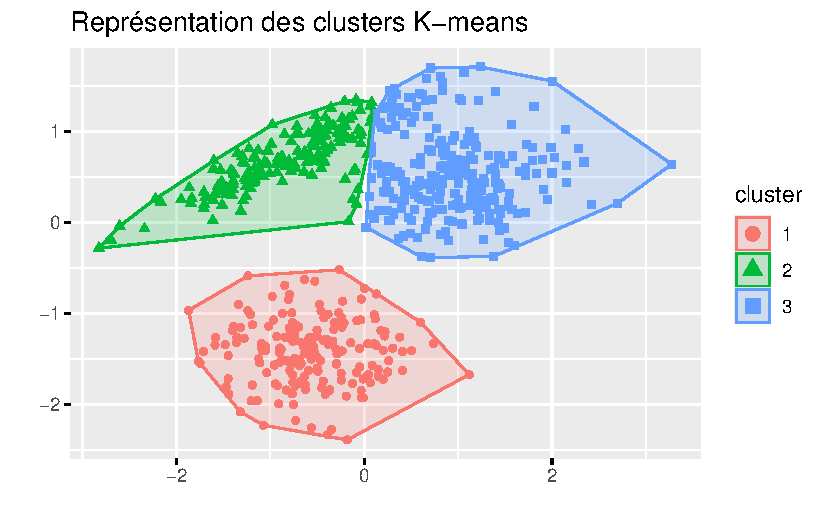
\includegraphics[keepaspectratio]{cluster_analysis_files/figure-pdf/unnamed-chunk-16-1.pdf}}

Cecie est un test

\protect\phantomsection\label{refs}
\begin{CSLReferences}{1}{1}
\bibitem[\citeproctext]{ref-clusterAnalysis}
Flynt, Abby, et Nema Dean. 2016. {«~A Survey of Popular R Packages for
Cluster Analysis~»}. \emph{Journal of Educational and Behavioral
Statistics} 41 (2): 205‑25.

\end{CSLReferences}




\end{document}
